\newcommand{\continuationNode}{
  node[draw=none]{} edge from parent[dashed,thin,-]
}

\newcommand{\rechercheAleatoireOne}{
  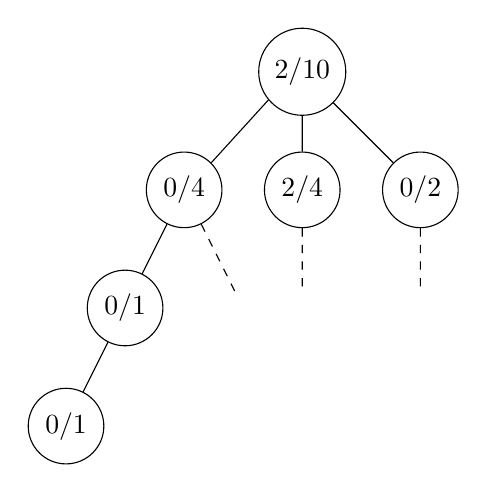
\begin{tikzpicture}[nodes={draw,circle}]
    \node{$2/10$}
      child{node{$0/4$}
        child{node{$0/1$}
          child{node{$0/1$}}
          child[missing]
        }
        child{\continuationNode}
      }
      child{node{$2/4$}
        child{\continuationNode}
      }
      child{node{$0/2$}
        child{\continuationNode}
      };
  \end{tikzpicture}
}

\newcommand{\rechercheAleatoireTwo}{
  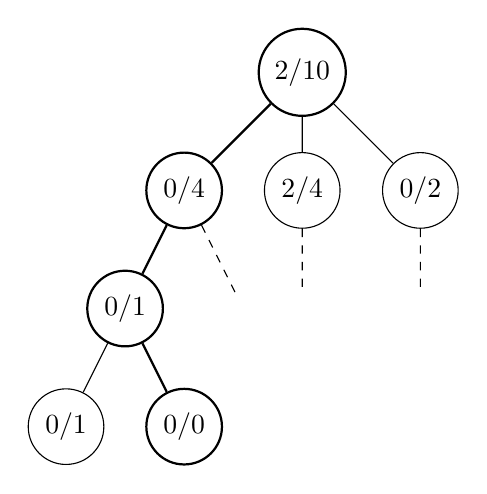
\begin{tikzpicture}[nodes={draw,circle}]
    \node[thick]{$2/10$}
      child{node[thick]{$0/4$}edge from parent[thick]
        child{node[thick]{$0/1$}edge from parent[thick]
          child{node[thin]{$0/1$}edge from parent[thin]}
          child{node[thick]{$\boldsymbol{0/0}$}edge from parent[thick]}
        }
        child{\continuationNode}
      }
      child{node{$2/4$}
        child{\continuationNode}
      }
      child{node{$0/2$}
        child{\continuationNode}
      };
  \end{tikzpicture}
}

\newcommand{\rechercheAleatoireThree}{
  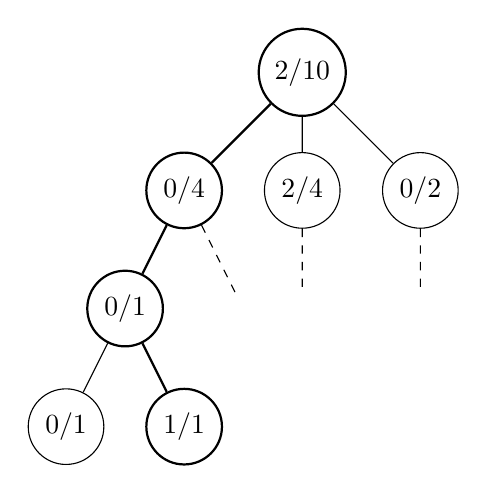
\begin{tikzpicture}[nodes={draw,circle}]
    \node[thick]{$2/10$}
      child{node[thick]{$0/4$}edge from parent[thick]
        child{node[thick]{$0/1$}edge from parent[thick]
          child{node[thin]{$0/1$}edge from parent[thin]}
          child{node[thick]{$\boldsymbol{1/1}$}edge from parent[thick]}
        }
        child{\continuationNode}
      }
      child{node{$2/4$}
        child{\continuationNode}
      }
      child{node{$0/2$}
        child{\continuationNode}
      };
  \end{tikzpicture}
}

\newcommand{\rechercheAleatoireFour}{
  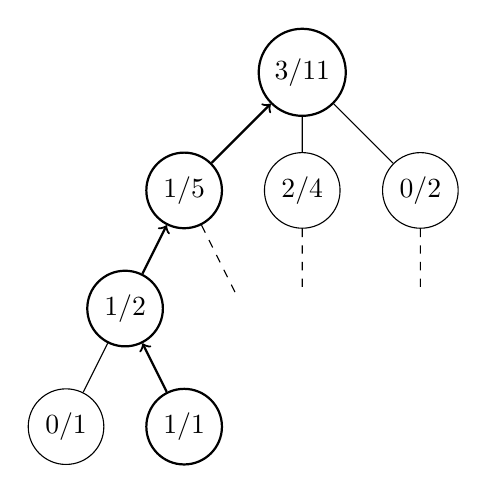
\begin{tikzpicture}[nodes={draw,circle}]
    \node[thick]{$3/11$}
      child{node[thick]{$1/5$}edge from parent[thick,<-]
        child{node[thick]{$1/2$}edge from parent[thick,<-]
          child{node[thin]{$0/1$}edge from parent[thin,-]}
          child{node[thick]{$\boldsymbol{1/1}$}edge from parent[thick,<-]}
        }
        child{\continuationNode}
      }
      child{node{$2/4$}
        child{\continuationNode}
      }
      child{node{$0/2$}
        child{\continuationNode}
      };
  \end{tikzpicture}
}


\begin{frame}
  \frametitle{Représentation sous forme d'arbre}
  \rechercheAleatoireOne
\end{frame}

\begin{frame}
  \frametitle{Représentation sous forme d'arbre}
  \rechercheAleatoireTwo
\end{frame}

\begin{frame}
  \frametitle{Représentation sous forme d'arbre}
  \rechercheAleatoireThree
\end{frame}

\begin{frame}
  \frametitle{Représentation sous forme d'arbre}
  \rechercheAleatoireFour
\end{frame}
